\section{Prototype Implementation}
\label{sec:implementation}


This section should provide brief details of how the prototype has been implemented.
You may want to use come code snippets here, but only focus on core features and aspects.
You are not meant to copy/paste your whole application code into the report.
Focus for instance how other developers may run your application and how they might develop it further...


The example below shows how you may include code. There are similar
styles for many other langages - in case you do not use Java in your
project. You can wrap the listing into a figure in case you need to
refer to it. How to create a figure was shown in Section~\ref{sec:technology}.

\lstinputlisting[language=java]{code/BoksVolum.java}

\subsection{Backend}

We will now look into how the Kotlin code is organized. We use Kotlin with Spring Boot as the backend. The code is organized into three main services: EventService, PollService, and UserService. These handle the business logic. We also have class JwtService,  which provides token management for authentication.
 
\vspace{1cm}

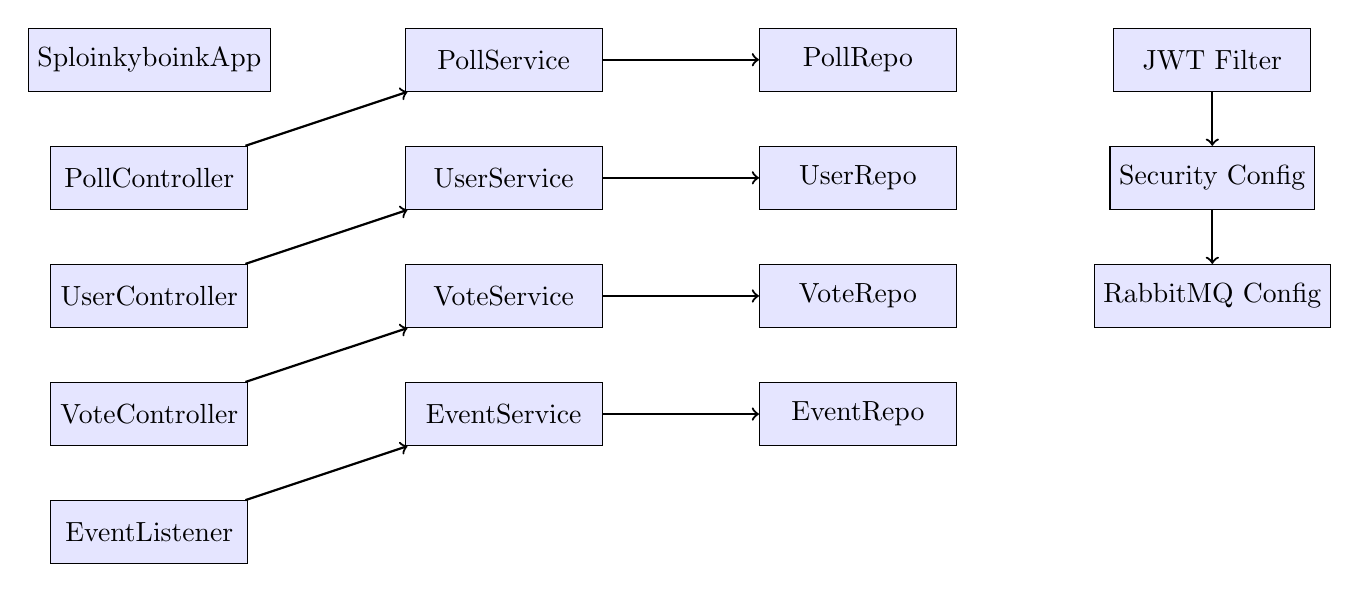
\begin{tikzpicture}[node distance=1.5cm]

% Define UML class styles
\tikzstyle{class} = [rectangle, draw=black, fill=blue!10, text centered, minimum height=0.8cm, minimum width=2.5cm]
\tikzstyle{arrow} = [->, thick, draw=black]

% Define nodes (classes)
\node[class] (sploinkyboinkApplication) {SploinkyboinkApp};
\node[class, below of=sploinkyboinkApplication] (pollController) {PollController};
\node[class, below of=pollController] (userController) {UserController};
\node[class, below of=userController] (voteController) {VoteController};
\node[class, below of=voteController] (eventListener) {EventListener};

% Define second layer nodes (Services)
\node[class, right of=sploinkyboinkApplication, xshift=3cm] (pollService) {PollService};
\node[class, below of=pollService] (userService) {UserService};
\node[class, below of=userService] (voteService) {VoteService};
\node[class, below of=voteService] (eventService) {EventService};

% Define third layer nodes (Repositories)
\node[class, right of=pollService, xshift=3cm] (pollRepository) {PollRepo};
\node[class, below of=pollRepository] (userRepository) {UserRepo};
\node[class, below of=userRepository] (voteRepository) {VoteRepo};
\node[class, below of=voteRepository] (eventRepository) {EventRepo};

% Define fourth layer nodes (Security)
\node[class, right of=pollRepository, xshift=3cm] (jwtAuthFilter) {JWT Filter};
\node[class, below of=jwtAuthFilter] (securityConfig) {Security Config};

% Define fifth layer nodes (Configurations)
\node[class, below of=securityConfig] (rabbitMQConfig) {RabbitMQ Config};

% Relationships (arrows)
\draw[arrow] (pollController) -- (pollService);
\draw[arrow] (userController) -- (userService);
\draw[arrow] (voteController) -- (voteService);
\draw[arrow] (eventListener) -- (eventService);

\draw[arrow] (pollService) -- (pollRepository);
\draw[arrow] (userService) -- (userRepository);
\draw[arrow] (voteService) -- (voteRepository);
\draw[arrow] (eventService) -- (eventRepository);

\draw[arrow] (jwtAuthFilter) -- (securityConfig);
\draw[arrow] (securityConfig) -- (rabbitMQConfig);

\end{tikzpicture}

\vspace{1cm}

\begin{itemize}
    \item \textbf{EventService}: Manages event logging, such as user votes and poll creation/editing.
    \item \textbf{PollService}: Handles poll management and voting logic.
    \item \textbf{UserService}: Manages user registration, authentication, and user data operations.
    \item \textbf{JwtService}: Provides token management for authentication.
    \item \textbf{Repositories}:The application uses repositories for data access (\texttt{PollRepo}, \texttt{UserRepo}, \texttt{VoteRepo}, \texttt{EventRepo}) and includes JWT filters for security, with RabbitMQ configured for message handling.
\end{itemize}

\vspace{0.5cm}

\textbf{Achieved functionalities}
\begin{itemize}
    \item \textbf{Polling Functionality}: Users can create, manage, and participate in polls, with their votes accurately captured and stored.
    \item \textbf{Event Tracking}: Tracks important user actions, enabling auditing or analytics.
    \item \textbf{User Management}: Ensures secure user authentication and management through validation mechanisms.
    \item \textbf{Integration with Messaging}: RabbitMQ integration supports a scalable, event-driven architecture, enabling the decoupling of services and enhancing overall application performance.
\end{itemize}


